% Provenance (never printed): see sources/outline_sources.md (Year 3:
% radial velocity, transits, imaging and microlensing; what has been
% found; atmospheres from transmission spectra).
% Brief: sources/book5/BRIEFS.md, ch. 28. Curves from figdata/bachelor-3/
% rv_transit.py (Keplerian radial-velocity curves, a limb-darkened transit
% light curve computed by numerical integration, point-lens microlensing)
% and exoplanet_archive.py (the NASA एक्सोप्लैनेट आर्काइव's composite table of
% confirmed planets, fetched 2026-10-23, with the model mass--radius curves
% of Zeng et al.). Exercise and problem values in the Book 5 scratch
% calculator calc/ch28.py. Selene's Lamp and its planet are invented.
\chapter{बहिर्ग्रह}\label{ch:b3:exoplanets}

1994 के शरद ऋतु में दो खगोलविदों ने 142
तारों के वेग मापते हुए पाया कि उनमें से एक, 51~पेगासी,
हमारी ओर और हमसे दूर गति करता है, लगभग चार दिन की अवधि के साथ। गति का अर्धआयाम
\qty{59}{m.s^{-1}} था, जो उनके स्पेक्ट्रोग्राफ़ से पता लगने योग्य मान से चार गुना था।
जिस साथी ने तारे को खींचकर घुमाया, उसका द्रव्यमान कम से कम
बृहस्पति का आधा था, और उसकी कक्षा \qty{0.05}{au} पर थी, जो उसके तारे से
बुध की सूर्य से दूरी से आठ गुना निकट है। ग्रह-निर्माण का कोई भी सिद्धांत
ऐसे पिंड के लिए स्थान नहीं रखता था। अक्तूबर 1995 में घोषित इस खोज ने खगोलविज्ञान का एक नया क्षेत्र खोल दिया:
तीन दशक बाद दूसरे तारों के चारों ओर छह हज़ार से अधिक ग्रहों की पुष्टि हो चुकी है,
उनमें से कुछ को सीधे देखा गया है, और कुछ के वायुमंडल का विश्लेषण किया गया है।
यह अध्याय दिखाता है कि इतने मंद ग्रह
कैसे खोजे जाते हैं, अब तक क्या मिला है,
और उनके वायुमंडल कैसे पढ़े जाते हैं।
% ledger: nobel19:51peg, planet:Mercury.dist, data:b5-pscomp

\begin{recall}
डॉप्लर प्रभाव, त्रिज्य वेग, स्पेक्ट्रमी द्वितारे, केपलर के
नियम, दो-पिंड समस्या और उसका द्रव्यमान-केंद्र, प्लांक का नियम और
समतापी वायुमंडल का मापनी ऊँचाई भौतिकी की पुस्तकों में हैं।
बहिर्ग्रह और तारे का वासयोग्य क्षेत्र विद्यालय की पुस्तकों में हैं।
किसी स्रोत का फ़्लक्स और दीप्ति पुस्तक 3 (स्नातक वर्ष 1) में, उसके दूरदर्शी और फ़ोटोमिति वाले
अध्याय में हैं; साम्य तापमान उसके तुलनात्मक ग्रहविज्ञान वाले अध्याय में है।
ग्रह-निर्माण और हिम रेखा पुस्तक 4 (स्नातक वर्ष 2) में हैं।
जीन्स और \omterm{def:b3:planetary-atmospheres:hydrodynamic}{जलगतिक पलायन} तथा वासयोग्य क्षेत्र की सीमाएँ
इस पुस्तक में, इसके ग्रहीय वायुमंडल वाले अध्याय में
हैं।
\end{recall}

\section{त्रिज्य-वेग विधि}\label{sec:b3:exoplanets:rv}

कोई ग्रह अपने तारे की परिक्रमा नहीं करता: दोनों अपने उभयनिष्ठ द्रव्यमान-केंद्र की परिक्रमा करते हैं।
तारा, जो कहीं अधिक भारी है, अपनी ही छोटी कक्षा में चलता है, और उसका प्रकाश
ग्रह की अवधि के साथ आगे-पीछे डॉप्लर-विस्थापित होता है।

\begin{definition}[त्रिज्य-वेग विधि; न्यूनतम द्रव्यमान]\label{def:b3:exoplanets:rv}
\emph{त्रिज्य-वेग विधि}\index{त्रिज्य-वेग विधि} किसी ग्रह को उसके तारे के
त्रिज्य वेग में आवर्ती परिवर्तन से पहचानती है,
जिसे तारे के स्पेक्ट्रम की रेखाओं के डॉप्लर विस्थापन से मापा जाता है। जब
कक्षा का आनति कोण $i$ आकाश-समतल से अज्ञात हो, तब यह
केवल ग्रह के द्रव्यमान और आनति कोण की ज्या के गुणनफल $m_p\sin i$ को मापती है,
जो ग्रह का \emph{न्यूनतम द्रव्यमान}\index{न्यूनतम द्रव्यमान}
है।
\end{definition}

\begin{theorem}[त्रिज्य-वेग अर्धआयाम]\label{thm:b3:exoplanets:semi-amplitude}
द्रव्यमान $M_\star$ का तारा और द्रव्यमान $m_p$ का ग्रह, वृत्ताकार कक्षा में,
आवर्त $P$ और आनति $i$ के साथ, तारे को त्रिज्य वेग
$v_r(t) = \gamma + K\cos\bigl(2\pi(t - t_0)/P\bigr)$ देते हैं, जहाँ $\gamma$ द्रव्यमान-केंद्र का
वेग है और अर्धआयाम
\[
K = \left(\frac{2\pi G}{P}\right)^{1/3}
    \frac{m_p\sin i}{(M_\star + m_p)^{2/3}} .
\]
है। विकेंद्रता $e$ की कक्षा पर वक्र अब ज्यावक्र नहीं रहता,
$v_r = \gamma + K\bigl[\cos(\nu + \omega) + e\cos\omega\bigr]$, जहाँ $\nu$
वास्तविक विषमकोण है और $\omega$ उपसौर-तर्क है, तथा $K$ का मान
$\sqrt{1 - e^2}$ से विभाजित होता है।
\end{theorem}

\begin{proof}
वृत्ताकार कक्षा के लिए: दोनों पिंडों की दूरी $a$ केपलर के तीसरे नियम का पालन करती है,
$a^3 = G(M_\star + m_p)P^2/4\pi^2$। तारा द्रव्यमान-केंद्र से
$a_\star = a\,m_p/(M_\star + m_p)$ दूरी पर स्थित है
और अपने वृत्त को चाल $v_\star = 2\pi a_\star/P$ से पूरा करता है। इसलिए
\[
v_\star = \frac{2\pi}{P}\,\frac{m_p}{M_\star + m_p}
          \left(\frac{G(M_\star + m_p)P^2}{4\pi^2}\right)^{1/3}
        = \left(\frac{2\pi G}{P}\right)^{1/3}\frac{m_p}{(M_\star + m_p)^{2/3}} .
\]
दृष्टि-रेखा कक्षा के समतल से $\pi/2 - i$ का कोण बनाती है,
इसलिए तारे के वेग का केवल $v_\star\sin i$ भाग उसके अनुदिश होता है, और
यह घटक तारे के साथ घूमता है: $v_r - \gamma = v_\star\sin i\,
\cos\bigl(2\pi(t - t_0)/P\bigr)$। विकेंद्रित रूप केपलर दीर्घवृत्त से
प्राप्त होता है और इसे स्वीकार किया जाता है।
\end{proof}

चूँकि ग्रह तारे से कहीं हल्का है, $K$ से $m_p\sin i$ निश्चित हो जाता है,
जब आवर्त मापा जा चुका हो और तारे का द्रव्यमान उसके
स्पेक्ट्रम से ज्ञात हो। 51~पेगासी~b के लिए $K = \qty{59}{m.s^{-1}}$ और $P = \qty{4.23}{d}$
एक सौर द्रव्यमान के तारे के चारों ओर $m_p\sin i = 0.47$ बृहस्पति द्रव्यमान प्राप्त होता है।
बृहस्पति सूर्य को \qty{12.5}{m.s^{-1}} से चलाता है, अपनी \num{4331}-दिन की
कक्षा में: किसी दूर के प्रेक्षक को सूर्य का वेग लगभग
\qty{\pm 13}{m.s^{-1}} तक बारह वर्षों में डोलता दिखेगा। पृथ्वी सूर्य को \qty{9}{cm.s^{-1}} से चलाती है।
जिस स्पेक्ट्रोग्राफ़ ने 51~पेगासी~b खोजा, उसकी सीमा \qty{13}{m.s^{-1}} थी;
उसके उत्तराधिकारी लगभग \qty{1}{m.s^{-1}} तक पहुँचते हैं (यानी \qty{3.5}{km/h} की पैदल चाल),
और सबसे नवीन यंत्र लगभग \qty{10}{cm.s^{-1}} के लिए बना है,
जो एक निम्न-द्रव्यमान तारे के वासयोग्य क्षेत्र में पृथ्वी-द्रव्यमान के ग्रह के लिए पर्याप्त है,
जहाँ ग्रह की कक्षा छोटी और उसका तारा कम द्रव्यमान का होता है।
तारा स्वयं एक निचली सीमा निर्धारित करता है: उसकी सतह के स्पंद और धब्बे,
जिन्हें उसका घूर्णन घुमाता रहता है, उसकी रेखाओं को भी विस्थापित करते हैं,
और ग्रह के संकेत को उनसे अलग पहचानना पड़ता है।
% ledger: nobel19:51peg, nobel19:sun-jupiter, nobel19:migration, planet:Jupiter.mass, planet:Jupiter.Porb, planet:Jupiter.ecc, planet:Earth.mass, sun:mass, eso:espresso, const:G

\begin{omfigure}
\centering
\begin{tikzpicture}
\begin{axis}[width=0.86\linewidth, height=0.40\linewidth,
  xmin=0, xmax=2, ymin=-40, ymax=42,
  xlabel={कक्षीय कला (आवर्तों में)}, ylabel={$v_r - \gamma$ (\unit{m.s^{-1}})},
  tick label style={font=\scriptsize}, label style={font=\small},
  legend style={font=\scriptsize, at={(0.5,-0.30)}, anchor=north, legend columns=2, draw=none, cells={anchor=west}, /tikz/every even column/.append style={column sep=1em}}]
\addplot[thin, black!40, forget plot] coordinates {(0,0) (2,0)};
\addplot[thick, omDef] table[x=phase, y=v_circ] {figdata/out/bachelor-3-rv_transit-rv.dat};
\addlegendentry{वृत्ताकार कक्षा}
\addplot[thick, dashed, red!70!black] table[x=phase, y=v_ecc] {figdata/out/bachelor-3-rv_transit-rv.dat};
\addlegendentry{$e = 0.3$, $\omega = \ang{60}$}
\draw[<->, thick] (axis cs:1.0,0) -- (axis cs:1.0,30);
\node[font=\scriptsize, anchor=east] at (axis cs:0.99,12) {$K$};
\end{axis}
\end{tikzpicture}
\par\smallskip{\small एक ग्रह वाले तारे का त्रिज्य वेग, दो
कक्षाओं पर, एक काल्पनिक ग्रह के लिए जिसका $K = \qty{30}{m.s^{-1}}$ और
आवर्त दस दिन का है। वृत्ताकार कक्षा (ठोस) पर वक्र अर्धआयाम
$K$ का ज्यावक्र है। विकेंद्रित कक्षा (बिंदीदार) पर तारा उपसौर के पास सबसे
तेज़ चलता है, और वक्र एक ओर झुक जाता है: उसके चरम मान
$K(1 \pm e\cos\omega)$ हैं और शिखर-से-शिखर विस्तार
$2K$ ही रहता है।}\label{fig:b3:exoplanets:rv}
\end{omfigure}

\section{पारगमन}\label{sec:b3:exoplanets:transits}

यदि कक्षा लगभग किनारे से देखी जाए, तो ग्रह अपने तारे के सामने से
हर कक्षा में एक बार गुज़रता है और उसकी तश्तरी का एक छोटा भाग ढक लेता है।

\begin{definition}[पारगमन विधि; पारगमन गहराई; संघट्ट प्राचल]\label{def:b3:exoplanets:transit}
\emph{पारगमन विधि}\index{पारगमन विधि} किसी ग्रह का संसूचन उसके तारे की
आवर्ती मंदता से करती है, जो तब होती है जब ग्रह तारकीय तश्तरी को पार करता है।
\emph{पारगमन गहराई}\index{पारगमन गहराई} $\delta$ पारगमन के दौरान तारे के फ़्लक्स में आई
भिन्नात्मक कमी है। \emph{संघट्ट
प्राचल}\index{संघट्ट प्राचल (पारगमन)} $b = a\cos i/R_\star$ ग्रह और तारे के केंद्रों के बीच की
न्यूनतम दूरी है, जो आकाश पर देखी जाती है,
तारीय त्रिज्या $R_\star$ की इकाइयों में मापी गई, उस कक्षा के लिए जिसकी
त्रिज्या $a$ और नति $i$ है।
\end{definition}

\begin{proposition}[पारगमन गहराई]\label{prop:b3:exoplanets:depth}
त्रिज्या $R_p$ का एक अंधकारमय ग्रह, जो समान चमक वाले किसी तारे के पूरे सामने हो,
गहराई $\delta = (R_p/R_\star)^2$ प्राप्त होती है।
\end{proposition}

\begin{proof}
ग्रह $\pi R_p^2$ क्षेत्रफल ढकता है, जो $\pi R_\star^2$ क्षेत्रफल की तश्तरी का भाग है,
जो हर जगह समान रूप से चमकीली है; फ़्लक्स उसी अनुपात में घटता है।
\end{proof}

बृहस्पति के सूर्य के सामने से गुज़रने पर वह \qty{1.06}{\percent} मंद होगा,
और पृथ्वी के गुज़रने पर \num{84} भाग प्रति मिलियन: पहली मंदता एक छोटे दूरदर्शी की पहुँच में है,
जबकि दूसरी के लिए ऐसा अंतरिक्ष दूरदर्शी चाहिए जो हज़ारों तारों को
वर्षों तक मापे। तारकीय तश्तरी हालाँकि समान नहीं होती।

\begin{definition}[किनारा-अंधकारन]\label{def:b3:exoplanets:limb}
\emph{किनारा-अंधकारन}\index{किनारा-अंधकारन} तारे की पृष्ठीय चमक का वह ह्रास है
जो तश्तरी के केंद्र से उसके किनारे, यानी लिंब, तक होता है।
लिंब के पास दृष्टि-रेखा तारे के वायुमंडल में तिरछी प्रवेश करती है
और ऊपरी, ठंडी परतों में इकाई प्रकाशिक गहराई तक पहुँचती है, जो कम उत्सर्जित करती हैं।
इसे प्रायः द्विघात नियम के रूप में लिखा जाता है, जहाँ $\mu = \cos\theta =
\sqrt{1 - r^2}$ और $r$ तश्तरी के केंद्र से तारीय त्रिज्याओं में दूरी है:
$I(\mu)/I(1) = 1 - u_1(1 - \mu) - u_2(1 - \mu)^2$।
\end{definition}

किनारा-अंधकारित तश्तरी के केंद्र के पास स्थित ग्रह औसत से अधिक चमकीला प्रकाश ढकता है
और पारगमन को गहरा बनाता है; किनारे के पास वह कम ढकता है। प्रकाश-वक्र का तल गोल होता है,
और उसके किनारे नरम पड़ जाते हैं। पारगमन की अवधि
में ज्यामिति समाहित होती है।

\begin{theorem}[पारगमन अवधि]\label{thm:b3:exoplanets:duration}
आवर्त $P$, त्रिज्या $a$ और नति $i$ वाली वृत्तीय कक्षा के लिए, जहाँ
$p = R_p/R_\star$ और \omterm{def:b3:exoplanets:transit}{संघट्ट प्राचल} $b$ के साथ, प्रथम
संपर्क से अंतिम संपर्क तक का समय है:
\[
T_{14} = \frac{P}{\pi}\arcsin\!\left(\frac{R_\star}{a}\,
          \frac{\sqrt{(1 + p)^2 - b^2}}{\sin i}\right),
\]
और दूसरे तथा तीसरे संपर्क के बीच का समय, जब ग्रह पूरी तरह तश्तरी के भीतर होता है,
पूरी तरह तश्तरी के भीतर होने पर $T_{23}$ उसी सूत्र से प्राप्त होता है, जिसमें
$1 - p$ को $1 + p$ के स्थान पर रखा जाता है।
\end{theorem}

\begin{proof}
मान लीजिए $\varphi = 2\pi t/P$ मध्य-पारगमन से गिनी गई कक्षीय कला है।
आकाश पर प्रक्षेपित करने पर, $x$ ग्रह के पथ के अनुदिश और $y$ उसके आर-पार लेते हुए,
ग्रह का केंद्र $x = a\sin\varphi$ और $y = a\cos i\cos\varphi$ पर
तारे के केंद्र से स्थित होता है। तारीय त्रिज्याओं में, वर्ग दूरी है:
\[
z^2 = \left(\frac{a}{R_\star}\right)^2(\sin^2\varphi + \cos^2 i\cos^2\varphi)
    = \left(\frac{a}{R_\star}\right)^2\sin^2 i\,\sin^2\varphi + b^2 .
\]
तश्तरियाँ बाहर से तब स्पर्श करती हैं जब $z = 1 + p$ हो,
$\sin\varphi = \sqrt{(1 + p)^2 - b^2}\,R_\star/(a\sin i)$ पर, और ये
मध्य-पारगमन के सापेक्ष सममित होती हैं। पारगमन कला $2\varphi$ तक चलता है, अर्थात
समय, यानी $2\varphi P/2\pi = P\varphi/\pi$। जब $z = 1 - p$ हो, तो तश्तरियाँ
भीतर से स्पर्श करती हैं।
\end{proof}

विस्तृत कक्षा के लिए आर्कसाइन लगभग अपना तर्क ही होता है: $T_{14} \approx (P/\pi)
(R_\star/a)\sqrt{(1 + p)^2 - b^2}$। केंद्रीय पारगमन सबसे लंबा चलता है; सतही
पारगमन, जिसमें $b$ लगभग $1 + p$ होता है, छोटा और V-आकार का होता है।
प्रकाश-वक्र पर $T_{14}$ और $T_{23}$ मापने से $b$ और $a/R_\star$ मिलते हैं, और इस प्रकार
नति भी: पारगमन वह $\sin i$ दूर कर देता है
जिसे त्रिज्य-वेग अज्ञात छोड़ देता है।

\begin{omfigure}
\centering
\begin{tikzpicture}[scale=0.92]
\shade[inner color=yellow!25, outer color=orange!70] (0,0) circle (2);
\draw[orange!70!black] (0,0) circle (2);
\draw[dashed, black!60] (-3.2,-0.6) -- (3.2,-0.6);
\draw[->, black!60] (2.5,-0.6) -- (3.2,-0.6) node[right, font=\scriptsize] {पथ};
\foreach \x in {-2.117, -1.697, 1.697, 2.117} {\fill[black] (\x,-0.6) circle (0.2);}
\node[font=\scriptsize] at (-2.117,-1.0) {1};
\node[font=\scriptsize] at (-1.697,-0.2) {2};
\node[font=\scriptsize] at (1.697,-0.2) {3};
\node[font=\scriptsize] at (2.117,-1.0) {4};
\fill[black] (0,0) circle (0.03);
\draw[<->, thick, omDef] (0,0) -- (0,-0.6) node[midway, left, font=\scriptsize] {$bR_\star$};
\draw[->] (0,0) -- (1.414,1.414) node[midway, above left, font=\scriptsize] {$R_\star$};
\end{tikzpicture}\hfill
\begin{tikzpicture}
\begin{axis}[width=0.52\linewidth, height=0.42\linewidth,
  xmin=-4, xmax=4, ymin=0.9855, ymax=1.0025,
  xlabel={मध्य-पारगमन से समय (h)}, ylabel={सापेक्ष फ़्लक्स},
  yticklabel style={/pgf/number format/fixed, /pgf/number format/precision=3},
  tick label style={font=\scriptsize}, label style={font=\small},
  legend style={font=\scriptsize, at={(0.5,-0.30)}, anchor=north, legend columns=1, draw=none, cells={anchor=west}, /tikz/every even column/.append style={column sep=1em}}]
\addplot[thick, omDef] table[x=t_h, y=flux_ld] {figdata/out/bachelor-3-rv_transit-transit.dat};
\addlegendentry{किनारा-अंधकारित तारा}
\addplot[thick, dashed, black!60] table[x=t_h, y=flux_uni] {figdata/out/bachelor-3-rv_transit-transit.dat};
\addlegendentry{एकसमान तारा}
\draw[densely dotted, black!50] (axis cs:-2.698,0.9855) -- (axis cs:-2.698,1.0025);
\node[font=\scriptsize, anchor=south] at (axis cs:-2.698,1.0005) {1};
\draw[densely dotted, black!50] (axis cs:-2.162,0.9855) -- (axis cs:-2.162,1.0025);
\node[font=\scriptsize, anchor=south] at (axis cs:-2.162,1.0005) {2};
\draw[densely dotted, black!50] (axis cs:2.162,0.9855) -- (axis cs:2.162,1.0025);
\node[font=\scriptsize, anchor=south] at (axis cs:2.162,1.0005) {3};
\draw[densely dotted, black!50] (axis cs:2.698,0.9855) -- (axis cs:2.698,1.0025);
\node[font=\scriptsize, anchor=south] at (axis cs:2.698,1.0005) {4};
\end{axis}
\end{tikzpicture}
\par\smallskip{\small बाएँ: $p = R_p/R_\star = 0.1$ वाला एक ग्रह अपने तारे की तश्तरी को
\omterm{def:b3:exoplanets:transit}{संघट्ट प्राचल} $b = 0.3$ पर पार करता है, चार
संपर्कों 1 से 4 तक; तश्तरी किनारे की ओर अधिक गहरी है। दाएँ: इसका प्रकाश-वक्र
$a/R_\star = 15$ और दस दिन के आवर्त पर, द्विघात \omterm{def:b3:exoplanets:limb}{किनारा-अंधकारन} गुणांकों
$u_1 = 0.40$, $u_2 = 0.25$ वाले तारे के लिए (ठोस) और एकसमान तारे के लिए
(बिंदीदार, गहराई ठीक $p^2 = 1\,\%$) परिकलित किया गया है।
संपर्कों 2 और 3 के बीच किनारा-अंधकारित वक्र गोल है, और
मध्य-पारगमन के पास $p^2$ से अधिक गहरा है।}\label{fig:b3:exoplanets:transit}
\end{omfigure}

\begin{proposition}[पारगमन प्रायिकता]\label{prop:b3:exoplanets:probability}
त्रिज्या $a$ की एक वृत्ताकार कक्षा पर यादृच्छिक रूप से अभिविन्यस्त एक ग्रह
अपने तारे का ($b < 1$ के साथ) $R_\star/a$ प्रायिकता से पारगमन करता है।
\end{proposition}

\begin{proof}
यादृच्छिक रूप से अभिविन्यस्त कक्षाओं के लिए $\cos i$ 0 और 1 के बीच एकसमान बंटित होता है।
ग्रह तब पारगमन करता है जब $b = (a/R_\star)\cos i < 1$ होता है, अर्थात
जब $\cos i < R_\star/a$ होता है, और यह प्रायिकता $R_\star/a$ के साथ घटित होता है।
\end{proof}

दूर का एक प्रेक्षक पृथ्वी को सूर्य का पारगमन करते हुए देखेगा, इसकी प्रायिकता
\qty{0.47}{\percent} है, और बृहस्पति के लिए \qty{0.09}{\percent}। एक पारगमन
सर्वेक्षण अपने देखे गए तारों के चारों ओर के ग्रहों में से केवल एक छोटा भाग देखता है,
और अधिकतर वे जो तारे के निकट हैं।

हर विधि अकेले कुछ छोड़ देती है। \omterm{def:b3:exoplanets:rv}{त्रिज्य-वेग विधि}
$m_p\sin i$ देती है; पारगमन $R_p/R_\star$ और $i$ देता है। दोनों मिलकर
सही द्रव्यमान और त्रिज्या देते हैं, और इसलिए माध्य घनत्व
$\bar\rho = 3m_p/4\pi R_p^3$ प्राप्त होता है, जो इस बात का पहला संकेत है कि ग्रह किससे बना है।
वर्ष 2000 के आरंभ में सूचित किए गए पहले पारगमन उस ग्रह के थे जो अपने तारे के वेग से
पहले ही ज्ञात था, HD~209458~b। उसके दो पारगमनों ने
तारे का \omterm{def:b3:exoplanets:limb}{किनारा-अंधकारन} दिखाया और 1.27 बृहस्पति त्रिज्या दी,
\ang{87.1} के झुकाव पर। अभिलेख के द्रव्यमान और त्रिज्या से इसका माध्य घनत्व
\qty{0.34}{g.cm^{-3}} है, जो जल के घनत्व का एक-तिहाई है: एक गैस दानव जो
अपने तारे की ऊष्मा से फूला हुआ है।
% ledger: planet:Jupiter.diameter, planet:Earth.diameter, sun:R, const:au, planet:Jupiter.dist, charbonneau00:hd209458, nobel19:transits, data:b5-pscomp

एक पारगमन करता ग्रह समय रखता है। यदि कोई दूसरा ग्रह उसे खींचता है, तो उसके
पारगमन ऐसे प्रतिरूप में जल्दी या देर से आते हैं जो
गुरुत्वीय अंतःक्रिया के साथ दोहराता है।

\begin{definition}[पारगमन-समय विचरण]\label{def:b3:exoplanets:ttv}
\emph{पारगमन-समय विचरण}\index{पारगमन-समय विचरण} किसी ग्रह के पारगमनों के समय का
कठोर आवर्ती क्रम से विचलन है,
तंत्र के किसी अन्य पिंड के गुरुत्वीय खिंचाव से उत्पन्न होता है;
यह उन ग्रहों को प्रकट कर सकता है और उनका द्रव्यमान माप सकता है,
जो स्वयं पारगमन नहीं करते।
\end{definition}

प्रकाश-वक्र में एक गिरावट हमेशा ग्रह नहीं होती। एक ग्रहण-युग्म, जिसके तारे केवल छूकर निकलते हैं,
या लक्ष्य के पीछे स्थित एक मंद ग्रहण-युग्म, जिसका प्रकाश
लक्ष्य के प्रकाश से तनु होता है, पारगमन की नकल कर सकता है। एक अभ्यर्थी तब
ग्रह बनता है जब उसका द्रव्यमान त्रिज्य-वेग से या समय-विचरणों से मापा जाए,
या जब हर अन्य व्याख्या खारिज कर दी गई हो।

\section{प्रत्यक्ष प्रतिबिंबन और सूक्ष्म-लेंसन}\label{sec:b3:exoplanets:imaging}

\begin{definition}[प्रत्यक्ष प्रतिबिंबन; कोरोनाग्राफ़]\label{def:b3:exoplanets:imaging}
\emph{प्रत्यक्ष प्रतिबिंबन}\index{प्रत्यक्ष प्रतिबिंबन} एक ग्रह को उसके अपने प्रकाश से संसूचित करता है,
जो परावर्तित या उत्सर्जित होता है और आकाश में अपने तारे के प्रकाश से
अलग दिखता है। \emph{कोरोनाग्राफ़}\index{कोरोनाग्राफ़} एक ऐसा उपकरण है जो
दूरदर्शी की नाभि पर तारे के प्रकाश को रोकता है, एक मास्क द्वारा या
प्रकाश के व्यतिकरण से, ताकि तारे के पास के मंद स्रोत
देखे जा सकें।
\end{definition}

इस कठिनाई के दो पहलू हैं। \qty{1}{au} की कक्षा, \qty{10}{pc} से देखी गई,
केवल \ang{;;0.1} फैलती है, और ग्रह अपने तारे से कई कोटि
मंद होता है। युवा विशाल ग्रह सबसे आसान लक्ष्य हैं: अपने निर्माण से अभी तक
तप्त होने के कारण वे अवरक्त में चमकते हैं, जहाँ
तारे के साथ उनका अंतर सबसे कम होता है। 2008 में दो बड़े दूरदर्शियों पर लिए गए चित्रों ने
तारे HR~8799 के चारों ओर तीन ग्रह दिखाए, जिनकी प्रक्षेपित दूरियाँ 24, 38 और
\qty{68}{au} थीं, और वे एक वर्ष से अगले वर्ष तक वामावर्त गति कर रहे थे; उनकी
कम दीप्ति और तंत्र की आयु उन्हें 5 से 13 बृहस्पति
द्रव्यमान देती हैं। नीचे के चित्र का ग्रह अपने तारे से \ang{;;0.82} दूर है;
अंतरिक्ष दूरदर्शी के \omterm{def:b3:exoplanets:imaging}{कोरोनाग्राफ़}
\num{1e-5} का अंतर \ang{;;1} पर और \qty{4.4}{\micro m} पर प्राप्त करते हैं।
% ledger: iau:parsec, const:au, marois08:hr8799, carter23:hip65426

\begin{omfigure}
\centering
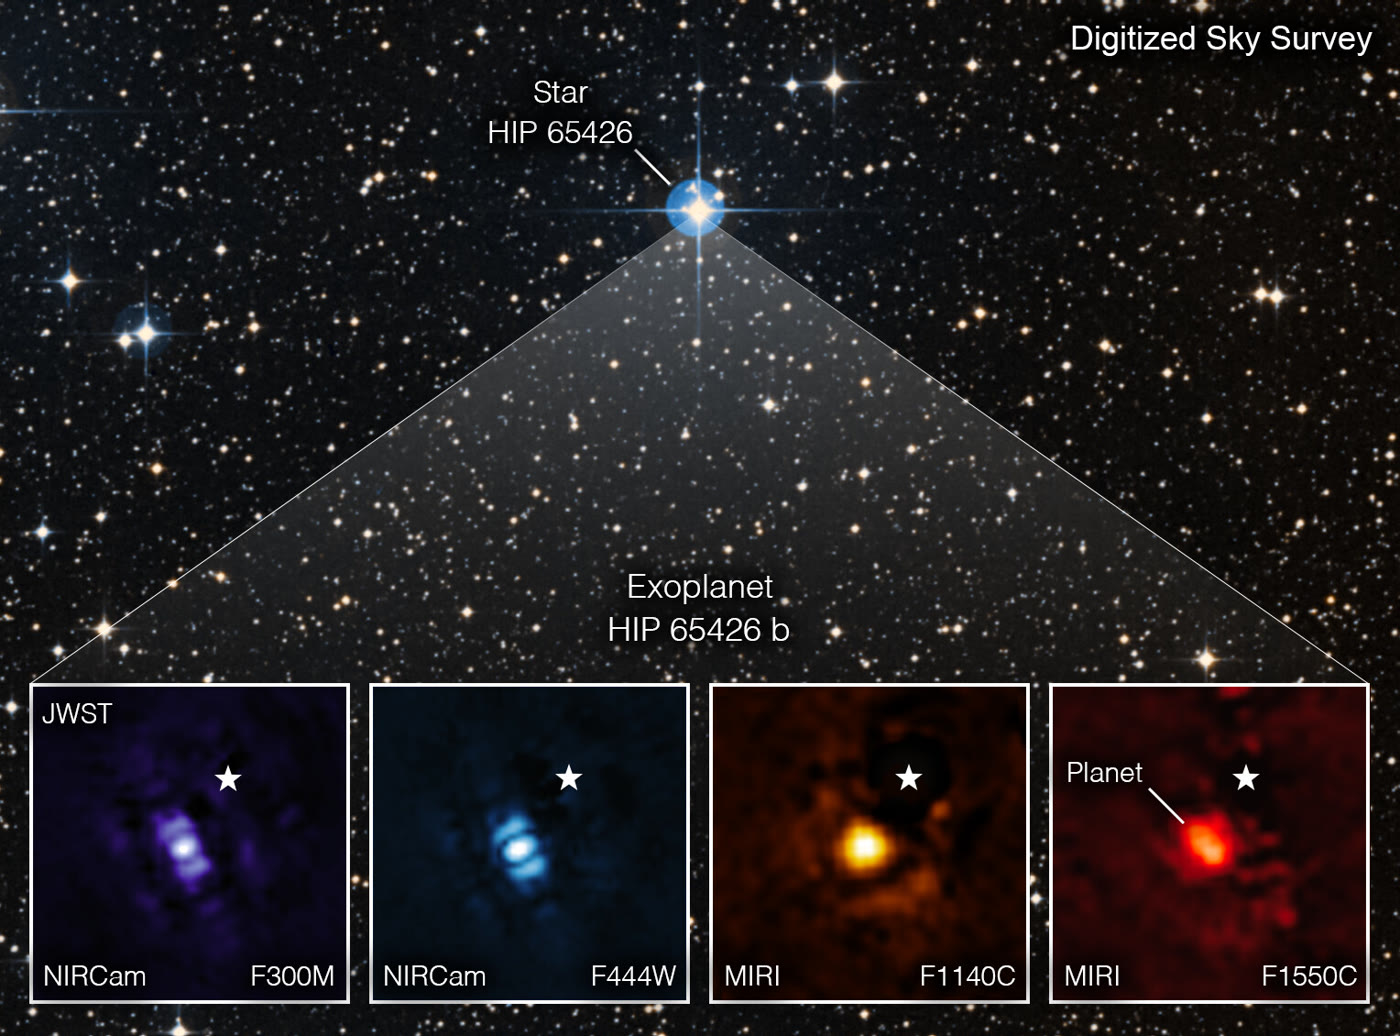
\includegraphics[width=0.86\linewidth]{images/book5/b3-hip65426b.jpg}
\par\smallskip{\small जेम्स वेब अंतरिक्ष दूरदर्शी द्वारा प्रतिबिंबित पहला बहिर्ग्रह,
HIP~65426~b, चार अवरक्त फ़िल्टरों में (नीचे; ऊपर,
भू-आधारित आकाश सर्वेक्षण में तारे का क्षेत्र); तारे का प्रकाश,
तारे के प्रतीक की स्थिति पर, तारे का प्रकाश
कोरोनाग्राफ़ों द्वारा रोका गया है। ग्रह लगभग 6 से 8 बृहस्पति द्रव्यमान का एक युवा गैस दानव है,
लगभग 15 से 20 मिलियन वर्ष पुराना, अपने तारे से लगभग सौ गुना
दूर है, जितना पृथ्वी सूर्य से है। चित्र NASA/ESA/CSA,
A~Carter (UCSC), ERS~1386 टीम, और A.~Pagan (STScI), CC
BY~4.0.}\label{fig:b3:exoplanets:hip65426}
\end{omfigure}
% ledger: photo:b3-hip65426b

एक चौथी विधि गुरुत्व को लेंस की तरह उपयोग करती है। जब एक तारा लगभग ठीक
किसी अधिक दूर के तारे के सामने से गुजरता है, तो उसका गुरुत्व पृष्ठभूमि तारे के प्रकाश को मोड़ता है
और उसे कुछ सप्ताह के लिए चमकीला कर देता है; लेंसिंग तारे का एक ग्रह
एक छोटा झटका जोड़ता है।

\begin{definition}[गुरुत्वीय सूक्ष्म-लेंसन; आइंस्टाइन त्रिज्या]\label{def:b3:exoplanets:microlensing}
\emph{गुरुत्वीय सूक्ष्म-लेंसन}\index{गुरुत्वीय सूक्ष्म-लेंसन} पृष्ठभूमि तारे की वह अस्थायी चमक है
जो तब होती है जब एक अग्रभूमि तारा, लेंस,
दृष्टि-रेखा के पास से गुजरता है; उसके बनाए प्रतिबिंब इतने पास होते हैं
कि उन्हें पृथक नहीं किया जा सकता। \emph{आइंस्टाइन त्रिज्या}\index{आइंस्टाइन त्रिज्या}
वह कोणीय त्रिज्या $\theta_\mathrm E$ है उस वलय की, जिसमें
द्रव्यमान $M$ वाला एक बिंदु-लेंस $D_L$ दूरी पर स्थित हो, तो वह
$D_S$ दूरी पर ठीक उसके पीछे स्थित एक स्रोत को मोड़ देगा:
\[
\theta_\mathrm E = \sqrt{\frac{4GM}{c^2}\,\frac{D_S - D_L}{D_L D_S}} .
\]
\end{definition}

\begin{proposition}[बिंदु-लेंस आवर्धन]\label{prop:b3:exoplanets:magnification}
बिंदु-लेंस से कोणीय दूरी $u\,\theta_\mathrm E$ पर स्थित एक स्रोत
इस गुणक से चमकीला हो जाता है:
\[
A(u) = \frac{u^2 + 2}{u\sqrt{u^2 + 4}} .
\]
\end{proposition}

\admitted

ये दोनों परिणाम किसी द्रव्यमान द्वारा प्रकाश के मुड़ने से आते हैं, जिसे सामान्य
आपेक्षिकता में समझाया जाता है। आधे सौर द्रव्यमान का एक लेंस, जो
\qty{8}{kpc} दूर स्रोत के ठीक बीच में हो, उसके लिए $\theta_\mathrm E = \qty{0.71}{mas}$ होता है, और लेंस की दूरी पर आइंस्टाइन
वलय की त्रिज्या \qty{2.9}{au} होती है। $u = 1$ पर
स्रोत की दीप्ति 1.34 गुना बढ़ती है, और $u = 0.1$ पर दस गुना। एक
ग्रह, जो अपने तारे के आइंस्टाइन वलय के निकट हो, प्रकाश वक्र में एक छोटा
विचलन जोड़ता है। इस प्रकार सूक्ष्म-लेंसन उन ग्रहों को खोजता है जो अपने तारों से
कुछ खगोलीय इकाइयों की दूरी पर होते हैं, वे शीतल ग्रह जिन्हें पारगमन और त्रिज्य-वेग नहीं पकड़ पाते,
किंतु प्रत्येक घटना केवल एक बार घटती है और दोहराई नहीं जाती। 2003 की एक घटना में,
जो अगले वर्ष प्रकाशित हुई, लगभग सात दिन तक रहने वाला एक विचलन केवल
ऐसे साथी द्वारा समझाया जा सका जिसका द्रव्यमान लेंस के द्रव्यमान का $\num{0.0039}$ गुना था:
लगभग 1.5 बृहस्पति द्रव्यमान का एक ग्रह, जो
अपने तारे से लगभग \qty{3}{au} दूर है।
% ledger: const:G, const:c, sun:mass, iau:parsec, const:au, bond04:ogle235

\begin{omfigure}
\centering
\begin{tikzpicture}[scale=0.95]
\fill (0,0) circle (0.06) node[below=2pt, font=\scriptsize] {स्रोत};
\fill[omDef] (3.2,0) circle (0.09); \node[font=\scriptsize, omDef] at (3.2,-1.15) {लेंस};
\draw[omDef] (3.2,0) ellipse (0.12 and 0.9);
\fill (6.4,0) circle (0.06) node[below=2pt, font=\scriptsize] {प्रेक्षक};
\draw[thick, orange!80!black] (0,0) -- (3.2,0.9) -- (6.4,0);
\draw[thick, orange!80!black] (0,0) -- (3.2,-0.9) -- (6.4,0);
\draw[densely dashed, black!50] (6.4,0) -- (0,1.8) node[left, font=\scriptsize] {प्रतिबिंब};
\draw[densely dotted, black!50] (0,0) -- (6.4,0);
\draw[<->] (3.55,0) -- (3.55,0.9) node[midway, right, font=\scriptsize] {$R_\mathrm E$};
\draw[<->, black!60] (0,-1.5) -- (3.2,-1.5) node[midway, below, font=\scriptsize] {$D_S - D_L$};
\draw[<->, black!60] (3.2,-1.5) -- (6.4,-1.5) node[midway, below, font=\scriptsize] {$D_L$};
\end{tikzpicture}\hfill
\begin{tikzpicture}
\begin{axis}[width=0.48\linewidth, height=0.42\linewidth,
  xmin=-3, xmax=3, ymin=0.8, ymax=12, ymode=log,
  ytick={1,2,5,10}, yticklabels={1,2,5,10},
  xlabel={समय ($t_\mathrm E$)}, ylabel={आवर्धन $A$},
  tick label style={font=\scriptsize}, label style={font=\small},
  legend style={font=\scriptsize, at={(0.5,-0.30)}, anchor=north, legend columns=3, draw=none, cells={anchor=west}, /tikz/every even column/.append style={column sep=1em}}]
\addplot[thick, omDef] table[x=t_tE, y=A01] {figdata/out/bachelor-3-rv_transit-lens.dat};
\addlegendentry{$u_0 = 0.1$}
\addplot[thick, dashed, red!70!black] table[x=t_tE, y=A03] {figdata/out/bachelor-3-rv_transit-lens.dat};
\addlegendentry{$0.3$}
\addplot[thick, dotted, black] table[x=t_tE, y=A10] {figdata/out/bachelor-3-rv_transit-lens.dat};
\addlegendentry{$1$}
\end{axis}
\end{tikzpicture}
\par\smallskip{\small बाईं ओर: गुरुत्वीय लेंस की ज्यामिति, पैमाने के अनुसार नहीं;
स्रोत से आने वाली किरणें लगभग \omterm{def:b3:exoplanets:microlensing}{आइंस्टाइन त्रिज्या} पर लेंस को पार करती हैं,
जो $R_\mathrm E = \theta_\mathrm E D_L$ है, और प्रेक्षक तक पहुँचती हैं, जिसे
स्रोत प्रतिबिंब की ओर विस्थापित दिखता है। दाईं ओर: बिंदु लेंस द्वारा बिंदु स्रोत का आवर्धन
समय के साथ, समय की इकाई $t_\mathrm E$ में, जिसमें लेंस
एक \omterm{def:b3:exoplanets:microlensing}{आइंस्टाइन त्रिज्या} भर चलने में लगता है, तीन निकटतम-दृष्टिकोण दूरियों
$u_0$ (आइंस्टाइन त्रिज्याओं में) के लिए।}\label{fig:b3:exoplanets:microlensing}
\end{omfigure}

हर विधि का अपना पूर्वाग्रह होता है, और ज्ञात ग्रहों की सूची
उन्हें प्रतिबिंबित करती है। त्रिज्य-वेग उन विशाल ग्रहों को अधिक खोजती है जो
अपने तारों के निकट हों; पारगमन बड़े ग्रहों को अधिक खोजता है, जो अपने तारों के निकट हों, और
उसके लिए कक्षा का किनारे से देखा जाना ज़रूरी है; सूक्ष्म-लेंसन कुछ खगोलीय इकाइयों की दूरी वाले ग्रह खोजता है;
प्रतिबिंबन दसियों या सैकड़ों खगोलीय इकाइयों दूर के युवा विशाल ग्रह खोजता है।
नीचे दिया चित्र परिणाम दिखाता है: प्रत्येक विधि अपना अलग क्षेत्र भरती है, और
सौरमंडल के ग्रह अधिकतर उनके बीच के अंतरालों में पड़ते हैं।

\begin{dated}{2026}
23 अक्टूबर 2026 को NASA एक्सोप्लैनेट आर्काइव में 6451 पुष्ट
ग्रह सूचीबद्ध थे। खोज की विधि के अनुसार: पारगमन से 4785, त्रिज्य-वेग से 1204,
सूक्ष्म-लेंसन से 292, प्रतिबिंबन से 98, \omterm{def:b3:exoplanets:ttv}{पारगमन-समय विचरण} से 29, और शेष
दुर्लभ विधियों से, जिनमें सबसे पहले ज्ञात ग्रह भी शामिल हैं,
जो 1992 में एक पल्सर के चारों ओर उसके स्पंदनों के समय से मिले थे। पहली
त्रिज्य-वेग द्वारा पहली खोजें 1995 से, पारगमन द्वारा 2002 से, सूक्ष्म-लेंसन
और प्रतिबिंबन द्वारा 2004 से हुईं।
\end{dated}
% ledger: data:b5-pscomp

\begin{omfigure}
\centering
\begin{tikzpicture}
\begin{axis}[width=0.86\linewidth, height=0.56\linewidth,
  xmode=log, ymode=log, xmin=0.004, xmax=2000, ymin=0.02, ymax=1e5,
  legend image post style={scale=2.2},
  xlabel={अर्ध-दीर्घ अक्ष (au)}, ylabel={द्रव्यमान या न्यूनतम द्रव्यमान ($M_\oplus$)},
  tick label style={font=\scriptsize}, label style={font=\small},
  legend style={font=\scriptsize, at={(0.5,-0.20)}, anchor=north, legend columns=4, draw=none, cells={anchor=west}, /tikz/every even column/.append style={column sep=1em}}]
\addplot[only marks, mark=*, mark size=0.6pt, omDef, opacity=0.6] table[x=a_au, y=mass] {figdata/out/bachelor-3-exoplanet_archive-ma-tr.dat};
\addlegendentry{पारगमन}
\addplot[only marks, mark=*, mark size=0.6pt, red!70!black, opacity=0.6] table[x=a_au, y=mass] {figdata/out/bachelor-3-exoplanet_archive-ma-rv.dat};
\addlegendentry{त्रिज्य-वेग}
\addplot[only marks, mark=triangle*, mark size=1.2pt, green!45!black] table[x=a_au, y=mass] {figdata/out/bachelor-3-exoplanet_archive-ma-ml.dat};
\addlegendentry{सूक्ष्म-लेंसन}
\addplot[only marks, mark=diamond*, mark size=1.5pt, orange!85!black] table[x=a_au, y=mass] {figdata/out/bachelor-3-exoplanet_archive-ma-im.dat};
\addlegendentry{प्रतिबिंबन}
\addplot[only marks, mark=square*, mark size=1.6pt, black, forget plot] table[x=a_au, y=mass] {figdata/out/bachelor-3-exoplanet_archive-solar.dat};
\node[font=\scriptsize, anchor=west, fill=white, inner sep=1pt] at (axis cs:1.15,1.0) {पृथ्वी};
\node[font=\scriptsize, anchor=east, fill=white, inner sep=1pt] at (axis cs:0.63,0.82) {शुक्र};
\node[font=\scriptsize, anchor=east, fill=white, inner sep=1pt] at (axis cs:0.34,0.055) {बुध};
\node[font=\scriptsize, anchor=west, fill=white, inner sep=1pt] at (axis cs:1.75,0.107) {मंगल};
\node[font=\scriptsize, anchor=west, fill=white, inner sep=1pt] at (axis cs:6.0,318) {बृहस्पति};
\node[font=\scriptsize, anchor=west, fill=white, inner sep=1pt] at (axis cs:11,95) {शनि};
\node[font=\scriptsize, anchor=north, fill=white, inner sep=1pt] at (axis cs:25,11) {यूरेनस, नेप्च्यून};
\end{axis}
\end{tikzpicture}
\par\smallskip{\small पुष्ट ग्रह, जिनका मापा गया द्रव्यमान (या \omterm{def:b3:exoplanets:rv}{न्यूनतम द्रव्यमान})
और अर्ध-दीर्घ अक्ष ज्ञात है, खोज की विधि के अनुसार (NASA एक्सोप्लैनेट
आर्काइव, 23 अक्टूबर 2026: पारगमन से 1691, त्रिज्य-वेग से 1151, सूक्ष्म-लेंसन से 286,
प्रतिबिंबन से 94), सौरमंडल के ग्रहों (काले
वर्ग) के साथ। \omterm{def:b3:exoplanets:mass-radius}{द्रव्यमान--त्रिज्या संबंध} से अनुमानित द्रव्यमान छोड़ दिए गए हैं। इस शोध में
NASA एक्सोप्लैनेट आर्काइव का उपयोग हुआ है, जिसका संचालन
California Institute of Technology करता है, जो राष्ट्रीय
वैमानिकी और अंतरिक्ष प्रशासन (NASA) के साथ अनुबंध में, एक्सोप्लैनेट एक्सप्लोरेशन
प्रोग्राम के अंतर्गत है।}\label{fig:b3:exoplanets:methods}
\end{omfigure}
% ledger: data:b5-pscomp, planet:Mercury.mass, planet:Venus.mass, planet:Earth.mass, planet:Mars.mass, planet:Jupiter.mass, planet:Saturn.mass, planet:Uranus.mass, planet:Neptune.mass, planet:Mercury.dist, planet:Venus.dist, planet:Earth.dist, planet:Mars.dist, planet:Jupiter.dist, planet:Saturn.dist, planet:Uranus.dist, planet:Neptune.dist

\section{जो पाया गया है}\label{sec:b3:exoplanets:found}

पहला आश्चर्य \omterm{def:b3:exoplanets:classes}{तप्त बृहस्पति} थे, ऐसे विशाल ग्रह जो
कुछ दिनों की कक्षाओं में घूमते हैं। 51~पेगासी~b अपने तारे के इतने पास नहीं बन सकता था; उसे
कहीं अधिक दूर बना होगा, शायद कुछ खगोलीय इकाइयों पर, अपनी चक्रिका की हिम रेखा के पार,
और चक्रिका के साथ अपनी अन्योन्य क्रिया से भीतर की ओर प्रवासित हुआ,
जैसा सिद्धांत ने पहले ही भविष्यवाणी की थी।
% ledger: nobel19:migration

\begin{definition}[तप्त बृहस्पति; अति-पृथ्वी; उप-नेपच्यून]\label{def:b3:exoplanets:classes}
\emph{तप्त बृहस्पति}\index{तप्त बृहस्पति} पास की कक्षा का एक विशाल ग्रह है,
जिसका \omterm{def:b3:exoplanets:rv}{न्यूनतम द्रव्यमान} सामान्यतः 0.1 बृहस्पति-द्रव्यमान से अधिक और आवर्तकाल
दस दिन से कम माना जाता है। \emph{अति-पृथ्वी}\index{अति-पृथ्वी} एक ऐसा ग्रह है
जो पृथ्वी से बड़ा पर \omterm{def:b3:exoplanets:radius-valley}{त्रिज्या घाटी} से छोटा है, अर्थात
लगभग 1.5 से 2 पृथ्वी-त्रिज्या तक, और इसलिए संभवतः चट्टानी। \emph{उप-नेपच्यून}\index{उप-नेपच्यून}
एक ऐसा ग्रह है जो \omterm{def:b3:exoplanets:radius-valley}{त्रिज्या घाटी} से ऊपर, पर नेप्च्यून से छोटा है, लगभग 2 से
4 पृथ्वी-त्रिज्या तक का, जिसकी त्रिज्या के लिए हल्की गैसों या
वाष्पशील पदार्थों का आवरण आवश्यक है।
\end{definition}
% ledger: wright12:hj, fulton17:gap, planet:Neptune.diameter, planet:Earth.diameter

\begin{definition}[उपस्थिति दर]\label{def:b3:exoplanets:occurrence}
किसी ग्रह-वर्ग की \emph{उपस्थिति दर}\index{उपस्थिति दर} वह है
प्रति तारे ऐसे ग्रहों की माध्य संख्या, या तारों का वह अंश जिनमें ऐसा एक ग्रह हो,
आकार (या द्रव्यमान) और आवर्तकाल की दी गई परास में, जब सर्वेक्षण की गिनतियों को
उन ग्रहों के लिए सुधारा जाए जिन्हें वह संसूचित नहीं कर सका:
वे जिनकी कक्षाएँ पारगमन के लिए संरेखित नहीं हैं, और वे
जो इतने छोटे या इतने दूर हैं कि दिखाई न दें।
\end{definition}

\omterm{def:b3:exoplanets:classes}{तप्त बृहस्पति}, जो सूची में प्रमुख हैं क्योंकि इन्हें सबसे आसानी से
खोजा जा सकता है, फिर भी दुर्लभ हैं: निकटवर्ती सूर्य-सदृश तारों के एक त्रिज्य-वेग सर्वेक्षण ने
इन्हें \qty[separate-uncertainty=true]{1.2 \pm 0.38}{\percent} तारों के आसपास पाया। छोटे ग्रह
आम हैं। केपलर अंतरिक्ष दूरबीन द्वारा देखे गए \num{42000} तारों के प्रकाश-वक्रों को खंगालने पर एक अध्ययन ने
603 ग्रह पाए, जिनमें से दस पृथ्वी के आकार के थे (1 से 2
पृथ्वी-त्रिज्या) जो पृथ्वी के सूर्यप्रकाश का एक से चार गुना प्राप्त करते थे;
पारगमन-प्रायिकता और उन ग्रहों के लिए संशोधित करने पर, जिन्हें खोज चूक जाती,
\qty[separate-uncertainty=true]{11 \pm 4}{\percent} सूर्य-सदृश तारों में
ऐसा एक ग्रह होता है।
% ledger: wright12:hj, petigura13:eta

छोटे ग्रहों के आकार समान रूप से वितरित नहीं हैं। पास की कक्षाओं वाले
सटीक मापे गए ग्रहों में, 1.5 से 2.0 पृथ्वी-त्रिज्या वाले ग्रह कम से कम दोगुने
दुर्लभ हैं, उनसे जो ठीक उससे छोटे या ठीक उससे बड़े हैं।

\begin{definition}[त्रिज्या घाटी]\label{def:b3:exoplanets:radius-valley}
\emph{त्रिज्या घाटी}\index{त्रिज्या घाटी} उन ग्रहों की कमी है
जिनकी त्रिज्या लगभग 1.5 और 2.0 पृथ्वी-त्रिज्या के बीच है, उन ग्रहों के बीच
जिनका आवर्तकाल लगभग सौ दिन से कम है; यह \omterm{def:b3:exoplanets:classes}{अति-पृथ्वी} को
\omterm{def:b3:exoplanets:classes}{उप-नेपच्यून} से अलग करती है।
\end{definition}
% ledger: fulton17:gap

इस घाटी को पलायन का चिह्न माना जाता है। एक चट्टानी क्रोड, जो जन्म से
हाइड्रोजन और हीलियम का, अपने द्रव्यमान के केवल कुछ प्रतिशत जितना आवरण लिए हो,
नंगे क्रोड से दोगुनी त्रिज्या रखता है। किसी युवा, सक्रिय तारे के निकट ऐसे
आवरण तप्त होकर \omterm{def:b3:planetary-atmospheres:hydrodynamic}{जलगतिक पलायन} द्वारा खो दिया जाता है:
पहले सौ मिलियन वर्षों में तारे के उच्च-ऊर्जा विकिरण से
(प्रकाश-वाष्पन), या ठंडे होते क्रोड की अपनी ऊष्मा से (क्रोड-संचालित
द्रव्यमान हानि)। मॉडल ग्रहों को लगभग 1.3 पृथ्वी-त्रिज्या के नंगे क्रोडों और
उससे दोगुने आकार के ग्रहों में समूहित कर देते हैं; बीच में कुछ ही बचते हैं।
ये दोनों क्रियाविधियाँ तारे पर भिन्न प्रकार से निर्भर करती हैं, और भिन्न प्रकार के तारों के
इर्द-गिर्द के ग्रह इन्हें अलग-अलग पहचानने में मदद कर सकते हैं।
% ledger: owen17:valley, ginzburg18:core-powered

\begin{omfigure}
\centering
\begin{tikzpicture}
\begin{axis}[name=pr, width=0.50\linewidth, height=0.50\linewidth,
  xmode=log, ymode=log, xmin=1, xmax=100, ymin=0.8, ymax=4,
  ytick={1,1.5,2,3,4}, yticklabels={1,1.5,2,3,4},
  xlabel={आवर्तकाल (दिन)}, ylabel={त्रिज्या ($R_\oplus$)},
  tick label style={font=\scriptsize}, label style={font=\small},
  title={(क)}, title style={font=\small}]
\fill[black!10] (axis cs:1,1.5) rectangle (axis cs:100,2.0);
\addplot[only marks, mark=*, mark size=0.5pt, omDef, opacity=0.7] table[x=period, y=radius] {figdata/out/bachelor-3-exoplanet_archive-pr.dat};
\end{axis}
\begin{axis}[at={(pr.east)}, anchor=west, xshift=0.09\linewidth,
  width=0.42\linewidth, height=0.50\linewidth,
  xmode=log, xmin=0.8, xmax=4, ymin=0, ymax=185,
  xtick={1,1.5,2,3,4}, xticklabels={1,1.5,2,3,4},
  xlabel={त्रिज्या ($R_\oplus$)}, ylabel={ग्रहों की संख्या},
  tick label style={font=\scriptsize}, label style={font=\small},
  title={(ख)}, title style={font=\small}]
\fill[black!10] (axis cs:1.5,0) rectangle (axis cs:2.0,185);
\addplot[const plot mark left, thick, omDef, fill=omDef!25] table[x=r, y=n] {figdata/out/bachelor-3-exoplanet_archive-histstep.dat} \closedcycle;
\end{axis}
\end{tikzpicture}
\par\smallskip{\small (क)~पारगमन करने वाले ग्रह, जिनकी त्रिज्या ज्ञात है
\qty{10}{\percent} से बेहतर, दो सौर-त्रिज्या से छोटे तारों के इर्द-गिर्द, जिनके
आवर्तकाल 1 से 100 दिन हैं (2370 ग्रह, NASA एक्सोप्लैनेट आर्काइव, 23
अक्टूबर 2026); छायांकित भाग 1.5 से 2.0 पृथ्वी-त्रिज्या की घाटी है।
(ख)~वही ग्रह, $\log R$ में समान चौड़ाई के 20 अंतरालों में गिने गए।
गिनतियाँ उन ग्रहों के लिए संशोधित नहीं हैं जिन्हें सर्वेक्षण छोड़ देते हैं, जो
छोटे ग्रहों में अधिक हैं; फिर भी घाटी दिखाई देती है।}\label{fig:b3:exoplanets:valley}
\end{omfigure}
% ledger: data:b5-pscomp, fulton17:gap

\begin{definition}[द्रव्यमान--त्रिज्या संबंध]\label{def:b3:exoplanets:mass-radius}
किसी संघटन का \emph{द्रव्यमान--त्रिज्या संबंध}\index{द्रव्यमान--त्रिज्या संबंध} वह
है जो उस संघटन के ग्रह की त्रिज्या को उसके द्रव्यमान के फलन के रूप में देता है,
जिसे उसकी सामग्रियों के अवस्था-समीकरणों से द्रवस्थैतिक साम्य में परिकलित किया जाता है;
एक मापे गए ग्रह की तुलना प्रत्याशी संघटनों के
संबंधों से की जाती है।
\end{definition}

एक चट्टानी ग्रह अपने ही भार से संपीड़ित होता है, और उसकी त्रिज्या
$M^{1/3}$ से धीमी बढ़ती है। पृथ्वी के भूकंपीय मॉडल पर आधारित दो-परत ग्रहों के मॉडलों
का एक फिट $R/R_\oplus = (1.07 - 0.21\,C)
(M/M_\oplus)^{1/3.7}$ देता है, 1 से 8 पृथ्वी-द्रव्यमान के लिए और क्रोड-द्रव्यमान अंश
$C$ 0 से 0.4 तक; पृथ्वी, शुक्र और कुछ छोटे
बहिर्ग्रहों पर फिट करने पर यह $C = 0.26 \pm 0.07$ देता है।
एक लौह ग्रह उसी द्रव्यमान पर छोटा होता है; आधा जल वाला ग्रह बड़ा;
केवल द्रव्यमान के दो प्रतिशत का हाइड्रोजन आवरण पाँच पृथ्वी-द्रव्यमान का ग्रह बनाता है
जिसका व्यास \num{2.6} पृथ्वी-त्रिज्या है, यानी
\omterm{def:b3:exoplanets:classes}{उप-नेपच्यून} का आकार। अपभ्रष्टता वास्तविक है: एक त्रिज्या और एक द्रव्यमान एक ही घनत्व देते हैं, और
लोहे, चट्टान, जल और गैस के कई मिश्रण उसे साझा कर सकते हैं।
चट्टानी ग्रह केप्लर-10~b, जो 3.24 पृथ्वी-द्रव्यमान और 1.47 पृथ्वी-त्रिज्या का है,
उसका माध्य घनत्व \qty{5.6}{g.cm^{-3}} है; गैस दानव WASP-39~b,
89 पृथ्वी-द्रव्यमान और 14.3 पृथ्वी-त्रिज्या वाला, उसका घनत्व \qty{0.17}{g.cm^{-3}} है।
% ledger: zeng16:rocky, data:b5-zeng, data:b5-pscomp

\begin{omfigure}
\centering
\begin{tikzpicture}
\begin{axis}[width=0.86\linewidth, height=0.58\linewidth,
  xmode=log, ymode=log, xmin=0.3, xmax=5000, ymin=0.5, ymax=25,
  ytick={0.5,1,2,4,10,20}, yticklabels={0.5,1,2,4,10,20},
  xlabel={द्रव्यमान ($M_\oplus$)}, ylabel={त्रिज्या ($R_\oplus$)},
  tick label style={font=\scriptsize}, label style={font=\small},
  legend style={font=\scriptsize, at={(0.5,-0.20)}, anchor=north, legend columns=3, draw=none, cells={anchor=west}, /tikz/every even column/.append style={column sep=1em}}]
\addplot[only marks, mark=*, mark size=0.6pt, black!35, forget plot] table[x=mass, y=radius] {figdata/out/bachelor-3-exoplanet_archive-mr.dat};
\addplot[thick, black] table[x=mass, y=radius] {figdata/out/bachelor-3-exoplanet_archive-zeng-iron.dat};
\addlegendentry{शुद्ध लोहा}
\addplot[thick, brown!70!black] table[x=mass, y=radius] {figdata/out/bachelor-3-exoplanet_archive-zeng-earthlike.dat};
\addlegendentry{पृथ्वी-जैसी चट्टान}
\addplot[thick, omDef] table[x=mass, y=radius] {figdata/out/bachelor-3-exoplanet_archive-zeng-water50.dat};
\addlegendentry{50\,\% जल}
\addplot[thick, dashed, orange!85!black] table[x=mass, y=radius] {figdata/out/bachelor-3-exoplanet_archive-zeng-h2-2pc.dat};
\addlegendentry{चट्टान + 2\,\% हाइड्रोजन}
\addplot[only marks, mark=square*, mark size=1.8pt, red!70!black] table[x=mass, y=radius] {figdata/out/bachelor-3-exoplanet_archive-solar.dat};
\addlegendentry{सौरमंडल}
\node[font=\scriptsize, anchor=north west] at (axis cs:1.05,0.97) {पृथ्वी};
\node[font=\scriptsize, anchor=south east] at (axis cs:0.80,0.97) {शुक्र};
\node[font=\scriptsize, anchor=south east, fill=white, inner sep=1pt] at (axis cs:13.5,4.3) {यूरेनस, नेपच्यून};
\node[font=\scriptsize, anchor=east, fill=white, inner sep=1pt] at (axis cs:80,9.45) {शनि};
\node[font=\scriptsize, anchor=north, fill=white, inner sep=1pt] at (axis cs:318,10.3) {बृहस्पति};
\end{axis}
\end{tikzpicture}
\par\smallskip{\small 1078 पारगमी ग्रहों का द्रव्यमान और त्रिज्या, जिनका
द्रव्यमान \qty{25}{\percent} से बेहतर और त्रिज्या
\qty{10}{\percent} से बेहतर मापा गया है (धूसर; NASA एक्सोप्लैनेट आर्काइव, 23 अक्टूबर 2026),
L.~Zeng और अन्य (2016, 2019) के मॉडल वक्रों के साथ: शुद्ध लोहा;
पृथ्वी-जैसी चट्टान, जिसमें एक-तिहाई लोहा और दो-तिहाई सिलिकेट है; ऐसे क्रोड पर आधा जल,
\qty{500}{K} पर; पृथ्वी-जैसा क्रोड, जिस पर हाइड्रोजन आवरण है,
जो उसके द्रव्यमान का \qty{2}{\percent} है, \qty{500}{K} पर। लाल वर्ग: सौरमंडल के
ग्रह (बुध और मंगल पैमाने से बाहर हैं, बाईं
ओर)।}\label{fig:b3:exoplanets:mass-radius}
\end{omfigure}
% ledger: data:b5-pscomp, data:b5-zeng, planet:Earth.mass, planet:Earth.diameter, planet:Venus.mass, planet:Venus.diameter, planet:Jupiter.mass, planet:Jupiter.diameter, planet:Saturn.mass, planet:Saturn.diameter, planet:Uranus.mass, planet:Uranus.diameter, planet:Neptune.mass, planet:Neptune.diameter

\section{वायुमंडल}\label{sec:b3:exoplanets:atmospheres}

पारगमी ग्रह को तौला और मापा जा सकता है; उसे सूँघा भी जा सकता है।
पारगमन के दौरान ग्रह के वायुमंडल की एक पतली वलय तारे के सामने खड़ी होती है,
और तारे का प्रकाश उसमें से छनकर निकलता है। जिन तरंगदैर्घ्यों पर वायुमंडल की कोई गैस
अवशोषण करती है, वहाँ वलय ऊपर की ओर अपारदर्शी हो जाती है,
और ग्रह बड़ा दिखता है।

\begin{definition}[पारगमन स्पेक्ट्रमिकी; द्वितीयक ग्रहण]\label{def:b3:exoplanets:transmission}
\emph{पारगमन स्पेक्ट्रमिकी}\index{पारगमन स्पेक्ट्रमिकी} \omterm{def:b3:exoplanets:transit}{पारगमन गहराई} को
तरंगदैर्घ्य के फ़ंक्शन के रूप में मापती है, ताकि
वायुमंडल की उन गैसों का संसूचन हो सके जिनसे तारे का प्रकाश ग्रह के किनारे पर होकर गुजरता है।
\emph{द्वितीयक ग्रहण}\index{द्वितीयक ग्रहण} किसी ग्रह का अपने तारे के पीछे से गुज़रना है, जो
वृत्ताकार कक्षा में पारगमन के आधे कक्षीय चक्र बाद होता है;
तब तंत्र के फ़्लक्स में आई गिरावट
ग्रह के दिवस-पक्ष के प्रकाश को मापती है।
\end{definition}

\begin{proposition}[पारगमन संकेत]\label{prop:b3:exoplanets:transmission}
पैमाना ऊँचाई $H \ll R_p$ वाला वायुमंडल, जो किसी अवशोषण पट्टी की तरंगदैर्घ्य पर
आस-पास की तरंगदैर्घ्यों की तुलना में $n$ अतिरिक्त पैमाना ऊँचाइयों तक अधिक अपारदर्शी हो,
वहाँ पारगमन को इतना गहरा करता है:
\[
\Delta\delta \approx n\,\frac{2HR_p}{R_\star^2} .
\]
\end{proposition}

\begin{proof}
ग्रह की आभासी त्रिज्या $R_p$ से बढ़कर $R_p + nH$ हो जाती है, इसलिए
गहराई $(R_p + nH)^2/R_\star^2$ में $(2nHR_p + n^2H^2)/R_\star^2$ की वृद्धि होती है,
जो $2nHR_p/R_\star^2$ के बराबर है, जब $nH \ll R_p$ हो।
\end{proof}

पैमाना ऊँचाई $H = kT/\bar m g$ एक गर्म, कम गुरुत्व वाले ग्रह के लिए बड़ी होती है जिसमें
हल्की हाइड्रोजन-वायु हो; एक ठंडे, घने ग्रह के लिए छोटी होती है जिसमें भारी वायु हो।
सूर्य के सामने देखी गई पृथ्वी के लिए, $H = \qty{8}{km}$ के साथ,
हर पैमाना ऊँचाई 0.2 भाग प्रति मिलियन जोड़ती है; एक गर्म, फूले हुए गैस दानव के लिए
कई सौ।
% ledger: planet:Earth.diameter, sun:R

\begin{proposition}[द्वितीयक-ग्रहण गहराई]\label{prop:b3:exoplanets:eclipse}
यदि किसी ग्रह का दिवस-पक्ष $T_d$ तापमान पर और तारा $T_\star$ पर
कृष्ण पिंड की भाँति विकिरण करे,
तो तरंगदैर्घ्य $\lambda$ पर \omterm{def:b3:exoplanets:transmission}{द्वितीयक ग्रहण} की गहराई होती है
\[
\delta_\mathrm{ecl} \approx \left(\frac{R_p}{R_\star}\right)^2
  \frac{B_\lambda(T_d)}{B_\lambda(T_\star)},
\]
जहाँ $B_\lambda$ प्लांक का नियम है और ग्रह के परावर्तित प्रकाश की उपेक्षा की गई है।
\end{proposition}

\begin{proof}
ग्रहण से ठीक पहले प्रेक्षक को तारे का प्रकाश प्राप्त होता है, जो $\pi R_\star^2 B_\lambda(T_\star)$
के अनुपात में है, साथ ही दिवस-पक्ष का, जो $\pi R_p^2 B_\lambda(T_d)$
के अनुपात में है; ग्रहण के दौरान केवल तारे का।
भिन्नात्मक गिरावट ग्रह के पद का तारे के पद से अनुपात है,
क्योंकि ग्रह का पद छोटा है।
\end{proof}

ग्रहण अवरक्त में सबसे गहरा होता है, जहाँ अपने तारे की तुलना में ठंडा ग्रह सबसे अधिक चमकीला होता है:
इससे दिवस-पक्ष का तापमान मिलता है, और एक गर्म दिवस-पक्ष, जिसके पास ठंडा रात्रि-पक्ष हो,
यह प्रकट करता है कि वायुमंडल पतला है या है ही नहीं,
जो ऊष्मा को इधर-उधर नहीं ले जाता।

\begin{dated}{2023}
2022 में गैस दानव WASP-39~b का पारगमन स्पेक्ट्रम,
जिसे जेम्स वेब स्पेस टेलीस्कोप ने 3.0 और \qty{5.5}{\micro m} के बीच मापा,
कार्बन डाइऑक्साइड की एक प्रमुख अवशोषण पट्टी
\qty{4.3}{\micro m} पर दिखाई, 26 मानक विचलन पर, जहाँ पहले की फ़ोटोमेट्री
केवल इस गैस का संकेत दे पाई थी: किसी बहिर्ग्रह के वायुमंडल में इसकी पहली स्पष्ट पहचान।
2023 में पाँच \omterm{def:b3:exoplanets:transmission}{द्वितीयक ग्रहण}, पृथ्वी-आकार के TRAPPIST-1~b के,
जो एक ठंडे, छोटे तारे से पृथ्वी के सूर्यप्रकाश का चार गुना पाता है,
\qty{15}{\micro m} पर मापे गए। वे
केवल दिवस-पक्ष से पुनर्विकिरित ऊष्मा से मेल खाते थे, बिना किसी
संसूचनीय कार्बन डाइऑक्साइड के, ग्रह के पास ऊष्मा को अपने रात्रि-पक्ष तक ले जाने के लिए
बहुत कम या कोई वायुमंडल है।
\end{dated}
% ledger: jwst23:wasp39-co2, greene23:trappist1b

छोटे तारों के वासयोग्य क्षेत्रों के चट्टानी ग्रह
इन विधियों की पहुँच में हैं, सीमा पर। क्या उन्होंने पिछले अध्याय की
पलायन प्रक्रियाओं के विरुद्ध अपना वायुमंडल बचाए रखा, यह अब एक
प्रेक्षणात्मक प्रश्न है।

\section{अभ्यास}

\begin{exercise}[$\star$]\label{exo:b3:exoplanets:1}
(क)~बृहस्पति (द्रव्यमान \qty{1898e24}{kg}, आवर्तकाल \num{4331}~दिन,
उत्केंद्रता 0.049) और पृथ्वी (द्रव्यमान \qty{5.97e24}{kg}, आवर्तकाल
\num{365.2}~दिन, उत्केंद्रता 0.017) के कारण सूर्य का त्रिज्य-वेग अर्ध-आयाम
परिकलित कीजिए। सूर्य का द्रव्यमान \qty{1.9884e30}{kg} है।
(ख)~परिशुद्धताओं \qty{3.5}{km/h} और \qty{0.35}{km/h} को
मीटर प्रति सेकंड में बदलकर तुलना कीजिए।
\end{exercise}

\begin{exercise}[$\star$]\label{exo:b3:exoplanets:2}
(क)~सूर्य (त्रिज्या \qty{695700}{km}) के पार बृहस्पति (त्रिज्या \qty{71492}{km})
और पृथ्वी (त्रिज्या \qty{6378}{km}) की \omterm{def:b3:exoplanets:transit}{पारगमन गहराई} परिकलित कीजिए। (ख)~एक
यादृच्छिक रूप से रखे गए प्रेक्षक द्वारा इनमें से प्रत्येक के पारगमन देखे जाने की
प्रायिकता परिकलित कीजिए, जब उनकी कक्षीय त्रिज्याएँ \num{778.5}
और \qty{149.6}{\mega km} हों।
\end{exercise}

\begin{exercise}[$\star$]\label{exo:b3:exoplanets:3}
51~पेगासी~b अपने तारे का त्रिज्य-वेग अर्ध-आयाम
\qty{59}{m.s^{-1}} देता है, जिसका आवर्तकाल \qty{4.23}{d} है। तारे का द्रव्यमान
सूर्य के बराबर मानकर, ग्रह का \omterm{def:b3:exoplanets:rv}{न्यूनतम द्रव्यमान} बृहस्पति द्रव्यमानों
और पृथ्वी द्रव्यमानों में, तथा उसकी कक्षा की त्रिज्या परिकलित कीजिए।
\end{exercise}

\begin{exercise}[$\star$]\label{exo:b3:exoplanets:4}
\qty{4}{kpc} पर स्थित आधे सौर द्रव्यमान का एक तारा, \qty{8}{kpc} पर
स्थित एक तारे को लेंस करता है ($\qty{1}{pc} = \qty{3.0857e16}{m}$)। (क)~लेंस की दूरी पर उसकी
\omterm{def:b3:exoplanets:microlensing}{आइंस्टाइन त्रिज्या} मिलिआर्कसेकंड में और आइंस्टाइन वलय की त्रिज्या खगोलीय इकाइयों में
परिकलित कीजिए। (ख)~$u = 1$, $0.5$ और $0.1$ पर आवर्धन परिकलित कीजिए।
(ग)~यदि लेंस रेखा-दृष्टि के पार
\qty{200}{km.s^{-1}} से गति करे, तो एक \omterm{def:b3:exoplanets:microlensing}{आइंस्टाइन त्रिज्या} पार करने में
उसे कितना समय लगेगा?
\end{exercise}

\begin{exercise}[$\star\star$]\label{exo:b3:exoplanets:5}
त्रिज्या अनुपात $p = 0.12$ वाला एक ग्रह एक सौर द्रव्यमान और एक सौर त्रिज्या वाले
तारे की \qty{3.0}{d} में परिक्रमा करता है। (क)~$a/R_\star$ परिकलित कीजिए। (ख)~$T_{14}$ और $T_{23}$
$b = 0$ और $b = 0.7$ के लिए परिकलित कीजिए, तथा दूसरी स्थिति में नति भी।
(ग)~प्रकाश वक्र का आकार केंद्रीय पारगमन को
स्पर्शी पारगमन से किस प्रकार अलग करता है?
\end{exercise}

\begin{exercise}[$\star\star$]\label{exo:b3:exoplanets:6}
एक्ज़ोप्लैनेट आर्काइव के द्रव्यमानों और त्रिज्याओं से TRAPPIST-1~b का (1.374 पृथ्वी
द्रव्यमान, 1.116 पृथ्वी त्रिज्या), केप्लर-10~b का (3.24, 1.47), WASP-39~b का
(89.31, 14.34) और HD~209458~b का (232.0,
15.58), $M_\oplus = \qty{5.97e24}{kg}$ और $R_\oplus =
\qty{6378}{km}$ लेकर माध्य घनत्व परिकलित कीजिए। कौन चट्टानी हैं और कौन गैसीय?
\end{exercise}

\begin{exercise}[$\star\star$]\label{exo:b3:exoplanets:7}
एक उत्केंद्र कक्षा में एक ग्रह वाले तारे का त्रिज्य-वेग
$+\qty{50.4}{m.s^{-1}}$ से $-\qty{9.6}{m.s^{-1}}$ तक परास रखता है, और तंत्र के
केंद्र-द्रव्यमान का वेग \qty{12.4}{m.s^{-1}} है। प्रमेय के उत्केंद्र रूप का उपयोग करके
$K$ और $e\cos\omega$ परिकलित कीजिए। दो चरम मानों का माध्य $\gamma$ से क्यों
भिन्न हो सकता है?
\end{exercise}

\begin{exercise}[$\star\star$]\label{exo:b3:exoplanets:8}
WASP-39~b का द्रव्यमान 89.31 पृथ्वी द्रव्यमान और त्रिज्या 14.34 पृथ्वी त्रिज्या है; उसके तारे की
त्रिज्या 0.939 सौर त्रिज्या है। वायुमंडल के लिए तापमान \qty{1100}{K} और औसत आणविक
द्रव्यमान \qty{2.3}{u} मान लीजिए। (क)~इसका गुरुत्व, मापनी ऊँचाई और \omterm{def:b3:exoplanets:transit}{पारगमन गहराई} परिकलित कीजिए।
(ख)~एक मापनी ऊँचाई और दो मापनी ऊँचाई ऊँचे अवशोषण बैंड का पारगमन संकेत,
दस लाख भागों में
परिकलित कीजिए।
\end{exercise}

\begin{exercise}[$\star\star$]\label{exo:b3:exoplanets:9}
TRAPPIST-1~b की त्रिज्या 1.116 पृथ्वी त्रिज्या है; उसका तारा, जिसकी त्रिज्या 0.1192 सौर
त्रिज्या और तापमान \qty{2566}{K} है। दिवस-पक्ष के \qty{400}{K} और \qty{500}{K} तापमानों पर
\qty{15}{\micro m} पर उसके \omterm{def:b3:exoplanets:transmission}{द्वितीयक ग्रहण} की गहराई
($hc/k = \qty{0.014388}{m.K}$) का प्रयोग करके परिकलित कीजिए। गहराई का मापन
किस प्रकार एक तापमापी है?
\end{exercise}

\begin{exercise}[$\star\star\star$]\label{exo:b3:exoplanets:10}
एक काल्पनिक लाल बौने तारे का द्रव्यमान 0.2 सौर द्रव्यमान, त्रिज्या 0.2 सौर
त्रिज्या और दीप्ति \num{0.005} सौर दीप्ति है। (क)~किस दूरी पर एक ग्रह को पृथ्वी का
तारकीय फ़्लक्स प्राप्त होता है, और उसका आवर्तकाल क्या है?
(ख)~वहाँ पृथ्वी द्रव्यमान के एक ग्रह के कारण उत्पन्न अर्ध-आयाम परिकलित करके,
उसकी तुलना पृथ्वी के सूर्य पर प्रभाव से कीजिए। (ग)~पृथ्वी-आकार के ग्रह की
\omterm{def:b3:exoplanets:transit}{पारगमन गहराई} परिकलित कीजिए। वासयोग्य क्षेत्रों में चट्टानी ग्रहों की खोज में
ऐसे तारे पसंदीदा लक्ष्य क्यों माने जाते हैं?
\end{exercise}

\begin{exercise}[$\star\star\star$]\label{exo:b3:exoplanets:11}
द्विघात \omterm{def:b3:exoplanets:limb}{किनारा-अंधकारन} नियम के लिए दिखाइए कि चकती की माध्य तीव्रता
$I(1)(1 - u_1/3 - u_2/6)$ है। निगमन द्वारा $p^2$ की इकाइयों में एक छोटे ग्रह की गहराई,
$r = 0$, $0.5$ और $0.9$ पर स्थित, $u_1 = 0.40$ और $u_2 = 0.25$ के लिए ज्ञात कीजिए।
एक समान-चकती मॉडल मध्य-पारगमन में प्रेक्षित ग्रह की त्रिज्या पर
$b = 0$ के लिए कौन-सी त्रुटि करेगा?
\end{exercise}

\begin{exercise}[$\star\star\star$]\label{exo:b3:exoplanets:12}
एक सर्वेक्षण ने \num{42000} सूर्य-सदृश तारों को देखा और उनमें ऐसे पृथ्वी-आकार के
ग्रहों की खोज की, जो पृथ्वी के सूर्यप्रकाश का एक से चार गुना प्राप्त करते हैं, अर्थात
0.5 से \qty{1}{au} तक की कक्षाओं में। (क)~0.5, 0.7 और \qty{1}{au} पर पारगमन
प्रायिकता परिकलित कीजिए। (ख)~यदि \qty{11}{\percent} तारों में
लगभग \qty{0.7}{au} पर ऐसा एक ग्रह हो, तो कितने पारगमन करेंगे?
(ग)~सर्वेक्षण में दस मिले। यह अंतर क्या मापता है, और
\omterm{def:b3:exoplanets:occurrence}{उपस्थिति दर} को इसके लिए सुधारना क्यों आवश्यक है?
\end{exercise}

\section{समस्या: सेलीन के दीपक के चारों ओर एक ग्रह}

\begin{problem}[{सप्ताहांत समस्या --- एक काल्पनिक ग्रह को तौलना, उसका आकार मापना
और उसके वायुमंडल को सूँघना}]
\label{pb:b3:exoplanets:1}
सेलीन का दीपक एक काल्पनिक K~वामन तारा है, जिसका द्रव्यमान 0.80 सौर द्रव्यमान,
त्रिज्या 0.76 सौर त्रिज्याएँ और प्रभावी तापमान \qty{5000}{K} है।
त्रिज्य-वेग सर्वेक्षण से पता चलता है कि इसका वेग ज्यावक्रीय रूप से
\qty{12.0}{d} की आवर्त-अवधि और \qty{2.59}{m.s^{-1}} के अर्ध-आयाम के साथ बदलता है। इसके बाद एक
अंतरिक्ष दूरदर्शी उसी आवर्त वाले पारगमन देखता है, जिनकी गहराई
\num{838} प्रति मिलियन भाग और कुल अवधि $T_{14} = \qty{3.23}{h}$ है।
मान लीजिए $M_\odot = \qty{1.9884e30}{kg}$, $R_\odot = \qty{695700}{km}$,
$L_\odot = \qty{3.828e26}{W}$, $M_\oplus = \qty{5.97e24}{kg}$,
$R_\oplus = \qty{6378}{km}$।

\medskip\noindent\textbf{भाग I --- त्रिज्य-वेग।}
\begin{enumerate}
\item ग्रह के द्रव्यमान को तारे के द्रव्यमान की तुलना में नगण्य मानते हुए,
  कक्षा की त्रिज्या मीटर और खगोलीय इकाइयों में परिकलित कीजिए।
\item ग्रह की कक्षीय चाल परिकलित कीजिए।
\item ग्रह का \omterm{def:b3:exoplanets:rv}{न्यूनतम द्रव्यमान} पृथ्वी के द्रव्यमानों में परिकलित कीजिए।
\item तारे की अपनी कक्षा की त्रिज्या, जो द्रव्यमान-केंद्र के परितः होती है,
  परिकलित कीजिए और जाँच कीजिए कि यह प्रेक्षित अर्ध-आयाम देती है।
\item संकेत \qty{1}{m.s^{-1}} की परिशुद्धता से कितने गुना अधिक है,
  और \qty{0.1}{m.s^{-1}} की परिशुद्धता से, यह ज्ञात कीजिए।
\item यदि कक्षा की उत्केंद्रता $e = 0.2$ हो और $K$ वही रहे, तो \omterm{def:b3:exoplanets:rv}{न्यूनतम द्रव्यमान}
  कितना बदलेगा, ज्ञात कीजिए।
\end{enumerate}

\medskip\noindent\textbf{भाग II --- पारगमन।}
\begin{enumerate}[resume]
\item त्रिज्या-अनुपात $p = R_p/R_\star$ परिकलित कीजिए।
\item ग्रह की त्रिज्या किलोमीटर में और पृथ्वी-त्रिज्याओं में परिकलित कीजिए।
\item $a/R_\star$ परिकलित कीजिए।
\item केंद्रीय पारगमन ($b = 0$) की अवधि परिकलित कीजिए।
\item प्रेक्षित $T_{14}$ से \omterm{def:b3:exoplanets:transit}{संघट्ट प्राचल} परिकलित कीजिए।
\item कक्षा का झुकाव-कोण परिकलित कीजिए।
\item यादृच्छिक दिशा से देखने पर इस ग्रह के पारगमन करने की
  प्रायिकता ज्ञात कीजिए।
\end{enumerate}

\medskip\noindent\textbf{भाग III --- यह किससे बना है?}
\begin{enumerate}[resume]
\item ग्रह का वास्तविक द्रव्यमान परिकलित कीजिए।
\item इसका माध्य घनत्व परिकलित कीजिए।
\item पृथ्वी-सदृश चट्टानी मॉडल वक्र पर इस द्रव्यमान के ग्रह की
  त्रिज्या 1.74 पृथ्वी-त्रिज्या होगी। तुलना कीजिए और बताइए कि ग्रह में
  चट्टान के अलावा और क्या होना चाहिए।
\item \omterm{def:b3:exoplanets:radius-valley}{त्रिज्या घाटी} के सापेक्ष ग्रह कहाँ स्थित है, ज्ञात कीजिए।
  और बताइए कि यह \omterm{def:b3:exoplanets:classes}{अति-पृथ्वी} है या \omterm{def:b3:exoplanets:classes}{उप-नेपच्यून}।
\item इसका पृष्ठ गुरुत्व परिकलित कीजिए।
\end{enumerate}

\medskip\noindent\textbf{भाग IV --- इसका वायुमंडल।}
\begin{enumerate}[resume]
\item तारे की दीप्ति वाट में और सौर दीप्तियों में
  परिकलित कीजिए।
\item ग्रह द्वारा प्राप्त तारकीय फ़्लक्स का, पृथ्वी के फ़्लक्स के सापेक्ष,
  परिकलित कीजिए। बताइए कि क्या यह वासयोग्य क्षेत्र में है।
\item बॉन्ड एल्बिडो 0.3 मानकर इसका साम्य तापमान परिकलित कीजिए।
\item हाइड्रोजन और हीलियम के वायुमंडल की पैमाना ऊँचाई
  (माध्य आणविक द्रव्यमान \qty{2.3}{u}) के साथ उस तापमान पर परिकलित कीजिए।
\item एक पैमाना ऊँचाई और दो पैमाना ऊँचाई ऊँचे जल-बैंड का पारगमन संकेत,
  प्रति मिलियन भाग में परिकलित कीजिए।
\item भाप के वायुमंडल (\qty{18}{u}) के लिए भी वही परिकलित कीजिए। इन दोनों में से
  कौन-सा, लगभग दस प्रति मिलियन भाग की परिशुद्धता वाला अंतरिक्ष दूरदर्शी,
  समतल स्पेक्ट्रम से अलग पहचान सकता है, बताइए।
\item ग्रह का माध्य घनत्व ग्राम प्रति घन सेंटीमीटर में,
  दो सार्थक अंकों तक दीजिए।
\end{enumerate}
\end{problem}
% ledger: sun:mass, sun:R, sun:L, planet:Earth.mass, planet:Earth.diameter, const:G, const:kB, const:sigma, nist:u, data:b5-zeng, fulton17:gap, eso:espresso
